\part{Ethernet-baseret Kommunikation}
\chapter{Industriel netværksprotokoller og standarder}	

\section{Modbus}
Modbus er en netværksprotokol med varianter for både seriel og TCP/IP-baseret kommunikation.

\paragraph{Modbus RTU:}
Modbus RTU (Remote Terminal Unit) er en seriel kommunikationsprotokol, der ofte bruges over RS-485-standarden. Den definerer, hvordan data pakkes i enheder kaldet frames og overføres mellem master- og slave-enheder.
\newline\newline 
\noindent\textbf{Protokol:} Modbus RTU beskriver, hvordan data formateres og adresseres inden for en ramme. Den definerer også mekanismer til fejldetektion og fejlkorrektion.
\newline\newline
\noindent\textbf{Elektrisk Standard:} Modbus RTU bruger elektriske standarder som RS-232, RS-422, og mest almindeligt, RS-485 for den fysiske transmission af data. RS-485 muliggør længere kabelafstande og understøtter multi-drop forbindelser.

\paragraph{Modbus TCP:}
Modbus TCP (Transmission Control Protocol) er en version af Modbus-protokollen, der kører over TCP/IP-netværk.
\newline\newline
\noindent\textbf{Protokol:} Modbus TCP definerer, hvordan Modbus-data pakkes inden for TCP/IP-rammer. Det muliggør kommunikation over Ethernet og bruger IP-adresser til at identificere enheder på netværket.
\newline\newline
\noindent\textbf{Elektrisk Standard:} Selvom Modbus TCP primært er en protokol, afhænger den af Ethernet's elektriske standarder for fysiske forbindelser. Dette inkluderer brug af Ethernet-kabler og standard netværksudstyr som switches og routers.

\subsection{Sammenfatning}
Både Profinet og Modbus (RTU og TCP) er primært protokoller, men de har også elektriske specifikationer og krav til det fysiske lag:
\begin{itemize}
	\item \textbf{Profinet:} En industriel Ethernet-protokol med specifikationer for elektriske standarder på det fysiske lag.
	\item \textbf{Modbus RTU:} En seriel protokol med tilknyttede elektriske standarder (RS-232, RS-422, RS-485).
	\item \textbf{Modbus TCP:} En TCP/IP-baseret protokol, der afhænger af Ethernet's elektriske standarder.
\end{itemize}
Dette afsnit understreger vigtigheden af at forstå både protokoller og elektriske standarder i industrielle netværk, hvilket er afgørende for at kunne designe og vedligeholde pålidelige og effektive kommunikationssystemer i industrielle miljøer.	

\subsection{Netværksprotokoller}
En netværksprotokol er et sæt regler og konventioner, der bestemmer, hvordan data udveksles mellem enheder som computere, smartphones, tablets og routere. Protokoller styrer flowet af bits mellem netværksinterfacekort, kontrollerer overførselshastigheden mellem sender og modtager, og bestemmer pakkernes vej fra kilde til destination.
\newline
\newline
\noindent For eksempel, når du anmoder om en webside ved at skrive en URL i din browser, sender din computer en forbindelsesanmodning til webserveren og venter på et svar. Webserveren svarer med en forbindelsesbekræftelse, hvorefter din computer sender en GET-besked med navnet på den ønskede side. Webserveren sender derefter den anmodede webside (fil) til din computer.
\newline
\newline
\noindent Protokoller definerer formatet og rækkefølgen af de beskeder, der udveksles, samt de handlinger, der udføres ved afsendelse eller modtagelse af en besked. De er essentielle for internet- og computernetværk, hvor nogle er simple og ligetil, mens andre er komplekse og dybdegående.
\newline
\newline
\noindent\textbf{Menneskelig analogi:}
Ligesom mennesker kommunikerer for at udveksle information, bruger netværksenheder protokoller til at udveksle data og styresignaler. Dette kan illustreres med et sekvensdiagram, hvor hver besked repræsenterer en del af kommunikationen mellem to parter. For eksempel kan en anmodning om tid sammenlignes med en TCP-anmodning om en fil.


\subsection{Elektriske Standarder}
Elektriske standarder definerer de fysiske egenskaber ved netværksforbindelser, såsom spændingsniveauer, signalstyrker, kabeltyper og stikforbindelser. Disse standarder sikrer, at de fysiske komponenter i netværket kan overføre data pålideligt.
\newline
\newline
\noindent Standarderne fastlægger, hvordan elektriske signaler skal behandles og transmitteres over netværket. Dette inkluderer specifikationer for voltagesvingninger, der styrer dataoverførsler, og hvor meget støj der kan tolereres uden at forstyrre signalet. For eksempel definerer Ethernet standarder for maksimale kabellængder og kabeltyper for at sikre, at signalerne forbliver stærke over lange afstande. USB-standarder specificerer typer af stik og kabler til data- og strømoverførsel.
\newline
\newline
\noindent Uden disse standarder ville der være betydelige kompatibilitetsproblemer mellem udstyr fra forskellige producenter, hvilket ville hæmme effektiv kommunikation og dataudveksling. Standarderne sikrer, at alle enheder på et netværk kan samarbejde effektivt, hvilket er afgørende for pålidelige og hurtige forbindelser i moderne kommunikationssystemer.
\newline
\newline
\noindent \textbf{Menneskelig analogi:}
Ligesom bygningsreglementer sikrer, at bygninger er sikre ved at specificere elektriske installationer, strukturel integritet og brandmodstand, sikrer elektriske standarder for netværk, at data kan overføres sikkert og effektivt. Bygningsstandarder sikrer kompatibilitet og sikkerhed, uanset hvilken entreprenør der udfører arbejdet. Tilsvarende garanterer netværksstandarder, at komponenter fra forskellige producenter kan arbejde sammen uden problemer, og at signaler kan transmitteres pålideligt over netværket.


\section{EtherNet/IP}
EtherNet/IP (Ethernet Industrial Protocol) er en avanceret industrielt netværksprotokol, der bygger på standard Ethernet-teknologi. Den bruges til at forbinde automatiseringsenheder som PLC'er, sensorer, aktuatorer og andre industrielle kontrolsystemer i realtid. EtherNet/IP er en af de mest udbredte netværksprotokoller i industriel automation og er kendt for sin fleksibilitet, skalerbarhed og høje ydeevne.

\subsection{Introduktion}
EtherNet/IP er udviklet til at understøtte både realtidsdataudveksling og ikke-realtids kommunikation i industrielle miljøer. Protokollen anvender standard TCP/IP og UDP/IP for at sikre kompatibilitet med eksisterende IT-netværk og tilbyder samtidig de nødvendige funktioner til at håndtere krævende industrielle applikationer, herunder motion control, procesautomation og sikkerhed.

\subsection{EtherNet/IP Protocol Stack}
EtherNet/IP-protokollen er opdelt i flere lag, hvor hvert lag håndterer specifikke funktioner i netværket. Denne lagdelte arkitektur tillader en høj grad af fleksibilitet og gør det muligt at implementere protokollen på forskellige typer hardware og i forskellige applikationer.

\subsection*{Fysisk Lag (Layer 1)}
Det fysiske lag i EtherNet/IP bygger på standard Ethernet-teknologi, hvilket betyder, at det understøtter brugen af standard Ethernet-kabler og stik (f.eks. Cat5e, Cat6). Dette lag definerer de elektriske og mekaniske egenskaber ved netværksforbindelserne og sikrer kompatibilitet med eksisterende Ethernet-infrastrukturer.

\subsection*{Datalink Lag (Layer 2)}
Datalink-laget i EtherNet/IP bygger på IEEE 802.3 Ethernet-standarden. Dette lag håndterer de grundlæggende funktioner for datatransmission, herunder adressering, rammeopbygning, fejlregistrering og fejlkontrol. Det sikrer pålidelig kommunikation mellem enheder på netværket.

\subsection*{Transport- og Netværkslag}
Transportlaget og netværkslaget i EtherNet/IP bruger standard TCP/IP- og UDP/IP-protokoller. TCP/IP bruges primært til ikke-realtids kommunikation, mens UDP/IP bruges til realtidskommunikation. Disse lag håndterer routingen af data gennem netværket og sikrer, at dataene leveres korrekt og i rette tid.

\subsection*{Applikationslag}
Applikationslaget i EtherNet/IP er baseret på Common Industrial Protocol (CIP). CIP definerer de dataobjekter, services og kommunikationsprotokoller, der bruges til at udføre specifikke opgaver som dataudveksling, kontrol og diagnostik. Dette lag muliggør interoperabilitet mellem enheder fra forskellige producenter.

\subsection*{Real-Time Communication}
EtherNet/IP understøtter både standard og realtidskommunikation. Real-time Communication (RTC) er en kritisk funktion for applikationer som motion control, hvor præcis timing og lav latenstid er nødvendigt. RTC opnås ved at anvende UDP/IP til at minimere kommunikationsforsinkelser.

\subsection{EtherNet/IP Kommunikationsmodel}
EtherNet/IP kommunikationsmodellen beskriver, hvordan data udveksles mellem enheder på netværket. Denne model understøtter både producer/consumer-modellen og client/server-modellen, hvilket giver stor fleksibilitet i, hvordan data struktureres og overføres.

\subsection{Forhold mellem Applikationsproces og Kommunikation}
Dette afsnit forklarer, hvordan applikationsprocesser interagerer med EtherNet/IP-protokollen for at sikre effektiv dataudveksling. Det beskriver, hvordan data fra applikationslaget omsættes til meddelelser, der kan sendes over netværket ved hjælp af CIP.

\subsection{Kommunikationsobjekter}
Kommunikationsobjekter i EtherNet/IP refererer til de enheder, data og tjenester, der adresseres og styres over netværket. Dette inkluderer en beskrivelse af forskellige typer af kommunikationsobjekter, såsom input/output-data, diagnostikbeskeder og konfigurationsdata, og deres anvendelse i forskellige scenarier.

\subsection{Ydeevne}
Dette afsnit diskuterer ydeevnen af EtherNet/IP-netværket, herunder dataoverførselshastigheder, latenstider og netværkskapacitet. Det giver også retningslinjer for optimering af netværksydeevne og sikring af, at systemet kan håndtere både realtids- og ikke-realtidskommunikation.

\subsection{Systemoperation}
\subsection*{Konfiguration}
Konfigurationen af et EtherNet/IP-netværk er afgørende for dets korrekte funktion. Dette afsnit beskriver trinene til at konfigurere enheder, tildele IP-adresser, og opsætte CIP-parametre, såsom prioriteringer og cyklustider for forskellige datatyper.

\subsection*{Dataoverførsel mellem PLC'er og Enheder}
Dette afsnit beskriver, hvordan data overføres mellem PLC'er og de tilsluttede enheder på netværket. Det inkluderer beskrivelser af cyclical data exchange og acyclic messaging, samt metoder til at sikre pålidelig dataudveksling.

\subsection*{Synkronisering og Timing}
Synkronisering og timing er afgørende for applikationer, der kræver præcis koordination mellem enheder, såsom i motion control. Dette afsnit forklarer, hvordan timingmekanismer implementeres i EtherNet/IP for at sikre nøjagtig dataoverførsel.

\subsection*{Sikkerhed og Netværksbeskyttelse}
Sikkerhed i EtherNet/IP-netværk er kritisk for at beskytte mod fejl og uautoriseret adgang. Dette afsnit beskriver de sikkerhedsforanstaltninger, der implementeres i EtherNet/IP, såsom autentificering, adgangskontrol, og kryptering for at beskytte dataoverførsel og enheder på netværket.

\subsection*{Integration med IT-systemer}
EtherNet/IP's basering på standard Ethernet og TCP/IP gør det velegnet til integration med eksisterende IT-systemer. Dette afsnit beskriver, hvordan EtherNet/IP kan anvendes sammen med enterprise-netværk, SCADA-systemer og andre IT-platforme for at skabe en fuldt integreret industriel løsning.

\subsection{Fejlfinding}
\subsection*{Introduktion}
Fejlfinding i et EtherNet/IP-netværk er en væsentlig del af vedligeholdelsen. Dette afsnit introducerer de grundlæggende metoder og principper for fejlfinding i EtherNet/IP-miljøer, herunder identifikation af almindelige problemer og deres løsninger.

\subsection*{Fejlfinding Værktøjer}
Der findes forskellige værktøjer til fejlfinding i EtherNet/IP-netværk. Dette afsnit beskriver nogle af de mest anvendte værktøjer, såsom netværksanalyzatorer, diagnostisk software og integrerede funktioner i Studio 5000, og hvordan de bruges til at identificere og løse problemer.

\subsection*{Tips}
Dette afsnit giver praktiske tips til optimering og vedligeholdelse af et EtherNet/IP-netværk. Tipsene inkluderer forebyggende foranstaltninger, overvågning af netværkets sundhed, og metoder til at undgå almindelige faldgruber i konfiguration og drift.

\subsection{Opsummering}
EtherNet/IP er en kraftfuld og fleksibel netværksprotokol, der er designet til at opfylde de komplekse krav i moderne industrielle automatiseringssystemer. Med sin evne til at håndtere realtidskommunikation, sikkerhed og integration med IT-systemer, er EtherNet/IP blevet en af de mest udbredte protokoller i industriel automation. Ved at forstå de forskellige aspekter af EtherNet/IP, fra protokolstacken til fejlfinding, kan teknikere og ingeniører sikre, at deres netværk fungerer optimalt og opfylder kravene til nutidens automatiseringsudfordringer.

\begin{figure}[!h]
	\centering
	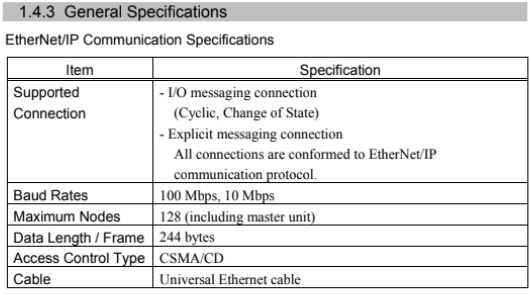
\includegraphics[width=\linewidth]{fig/fig16}
\end{figure}
\clearpage

\section{PROFINET}
PROFINET (Process Field Network) er en moderne, industrielt netværksprotokol, der muliggør hurtig og pålidelig kommunikation mellem automatiseringskomponenter, såsom PLC'er, sensorer, aktuatorer og HMI'er. PROFINET er udviklet som en efterfølger til ProfiBus, med fokus på Ethernet-baseret kommunikation og støtte til realtidsdataudveksling i komplekse industrielle miljøer.

\subsection{Introduktion}
PROFINET er designet til at imødekomme kravene i moderne automatiseringssystemer, hvor der er behov for højhastighedskommunikation, integration med IT-systemer og understøttelse af avancerede funktioner som sikkerhed og trådløs kommunikation. Protokollen gør det muligt at forbinde og styre en bred vifte af industrielle enheder i realtid, hvilket gør den ideel til både fabriksautomatisering og processtyring.

\subsection{PROFINET Protocol Stack}
PROFINET-protokollen er opdelt i flere lag, der hver især håndterer forskellige aspekter af kommunikationen. Denne strukturerede tilgang sikrer, at forskellige funktioner kan integreres og udføres effektivt inden for det samme netværk.

\subsection*{Fysisk Lag (Layer 1)}
Det fysiske lag i PROFINET er baseret på standard Ethernet-teknologi, hvilket betyder, at det understøtter standardiserede Ethernet-kabler og stik (f.eks. Cat5e, Cat6) og tilbyder høj båndbredde og fleksibilitet i netværksdesign. Dette lag specificerer også kravene til signalering og elektriske egenskaber.

\subsection*{Datalink Lag (Layer 2)}
Datalink-laget i PROFINET bygger på Ethernet MAC-laget, men tilføjer protokoltilpasninger, der understøtter realtidskommunikation (RT) og isokron realtidskommunikation (IRT). Dette lag håndterer pålidelig datatransmission, fejldetektion, adressering af enheder og datarammer.

\subsection*{Applikationslag}
Applikationslaget i PROFINET omfatter protokoller og tjenester, der er nødvendige for at implementere specifikke funktioner såsom procesdataudveksling, alarmer og diagnostik. Dette lag er også ansvarligt for konfiguration og parameterisering af enhederne på netværket.

\subsection*{Real-Time Communication (RT)}
RT-funktionen i PROFINET muliggør overførsel af procesdata med minimal latenstid, hvilket er afgørende for tidskritiske applikationer. RT kan håndtere periodiske og applikationsbestemte cykliske dataoverførsler.

\subsection*{Isocronous Real-Time Communication (IRT)}
IRT er en avanceret funktion i PROFINET, der gør det muligt at synkronisere dataoverførsel med en meget præcis timing, hvilket er nødvendigt i applikationer som motion control, hvor selv små forsinkelser kan føre til fejl.

\subsection{PROFINET Kommunikationsmodel}
PROFINET kommunikationsmodellen beskriver, hvordan data udveksles mellem enheder på netværket, inklusive de forskellige kommunikationscyklusser og dataoverførselshastigheder. Modellen understøtter både realtids- og ikke-realtidskommunikation, hvilket gør det muligt at kombinere proces- og konfigurationsdata på samme netværk.

\subsection{Forhold mellem Applikationsproces og Kommunikation}
Dette afsnit forklarer, hvordan applikationsprocesser interagerer med PROFINET-kommunikationsprotokollen for at sikre effektiv dataudveksling. Det beskriver, hvordan data struktureres og sendes mellem forskellige lag i protokolstacken for at opnå optimal kommunikationsperformance.

\subsection{Kommunikationsobjekter}
Kommunikationsobjekter i PROFINET refererer til de enheder, data og tjenester, der adresseres og styres over netværket. Dette afsnit inkluderer en beskrivelse af forskellige typer af kommunikationsobjekter, såsom input/output-data, alarmer og diagnostikbeskeder, og deres anvendelse i forskellige scenarier.

\subsection{Ydeevne}
Dette afsnit diskuterer ydeevnen af PROFINET-netværket, herunder dataoverførselshastigheder, latenstider og netværkskapacitet. Det indeholder også retningslinjer for optimering af netværkets ydeevne og sikring af, at systemet kan håndtere både realtids- og isokron dataoverførsel.

\subsection{Systemoperation}
\subsection*{Konfiguration}
Korrekt konfiguration er afgørende for at sikre, at PROFINET-netværket fungerer optimalt. Dette afsnit beskriver trinene til at konfigurere enheder, tildele IP-adresser og opsætte PROFINET-parametre, såsom cyklustider og prioriteter for forskellige datatyper.

\subsection*{Dataoverførsel mellem PLC'er og Enheder}
Dette afsnit beskriver, hvordan data overføres mellem PLC'er og de tilsluttede enheder på netværket. Det inkluderer beskrivelser af cyklisk og acyklisk dataoverførsel samt metoder til at sikre pålidelig dataudveksling.

\subsection*{Synkronisering og Timing}
Synkronisering og timing er centrale elementer i PROFINET-netværk, især i applikationer, der kræver præcis timing og koordinering mellem enheder. Dette afsnit forklarer, hvordan IRT og andre synkroniseringsmetoder implementeres i PROFINET.

\subsection*{Sikkerhed og Netværksbeskyttelse}
Sikkerhed i PROFINET-netværk er kritisk for at beskytte mod fejl og uautoriseret adgang. Dette afsnit beskriver de sikkerhedsforanstaltninger, der implementeres i PROFINET, såsom adgangskontrol, dataautentificering og kryptering.

\subsection*{Integration med IT-systemer}
Et af PROFINET's styrker er dets evne til at integrere med eksisterende IT-systemer. Dette afsnit beskriver, hvordan PROFINET kan anvendes sammen med enterprise-netværk, SCADA-systemer og andre IT-platforme for at skabe en fuldt integreret industriel løsning.

\subsection{Fejlfinding}
\subsection*{Introduktion}
Fejlfinding i et PROFINET-netværk er en essentiel del af vedligeholdelsen. Dette afsnit introducerer de grundlæggende metoder og principper for fejlfinding i PROFINET-miljøer, herunder de mest almindelige problemer og deres løsninger.

\subsection*{Fejlfinding Værktøjer}
Der findes en række værktøjer til fejlfinding i PROFINET-netværk. Dette afsnit beskriver nogle af de mest anvendte værktøjer, som netværkssniffere, diagnostiske software og integrerede funktioner i TIA Portal, og hvordan de anvendes til at identificere og løse problemer.

\subsection*{Tips}
Dette afsnit giver praktiske tips til optimering og vedligeholdelse af et PROFINET-netværk. Tipsene inkluderer forebyggende foranstaltninger, overvågning af netværkets sundhed, og metoder til at undgå almindelige faldgruber i konfiguration og drift.

\subsection{Opsummering}
PROFINET er en kraftfuld og fleksibel netværksprotokol, der er designet til at opfylde de komplekse krav i moderne industrielle automatiseringssystemer. Med sin evne til at håndtere realtidskommunikation, sikkerhed og integration med IT-systemer, er PROFINET blevet en af de mest anvendte protokoller i industriens 4.0 æra. Ved at forstå de forskellige aspekter af PROFINET, fra protokolstacken til fejlfinding, kan teknikere og ingeniører sikre, at deres netværk fungerer optimalt og opfylder kravene til nutidens automatiseringsudfordringer.

\section{AS-Interface (AS-i) Overview}
AS-Interface (AS-i) er en simpel og effektiv feltbusløsning designet til at forbinde sensorer og aktuatorer i automatiseringssystemer. AS-i er kendt for sin nemme installation og vedligeholdelse, hvilket gør det til et populært valg i industrielle applikationer.

\subsection{Introduktion}
AS-i blev udviklet som en økonomisk og brugervenlig måde at forbinde enheder som sensorer, aktuatorer og PLC'er (Programmable Logic Controllers). AS-i er kendetegnet ved en to-leder fladkabel teknologi, som både overfører data og leverer strøm til tilsluttede enheder. Denne enkelhed gør det muligt for AS-i at reducere omkostningerne og kompleksiteten ved installation og vedligeholdelse.

\subsection{Layer 1 – The Physical Layer}
Det fysiske lag i AS-i definerer de elektriske og mekaniske egenskaber ved netværksforbindelserne. Dette inkluderer specifikationer for kabler, stik og elektriske signaler, der bruges til at overføre data og strøm mellem enheder. AS-i bruger et fladkabelsystem, som er nemt at installere og tilslutte, hvilket minimerer fejl og reducerer installationsomkostningerne.

\subsection{Layer 2 – The Data Link Layer}
Datalink-laget håndterer pålidelig overførsel af data mellem enheder på AS-i netværket. Dette lag sikrer korrekt adressering, fejlregistrering og dataintegritet ved hjælp af cyklisk redundanskontrol (CRC). Datalink-laget koordinerer også kommunikationen mellem master- og slaveenheder, hvilket sikrer synkroniseret dataudveksling.

\subsection{Operating Characteristics}
AS-i systemet er designet til at fungere under forskellige industrielle forhold og tilbyder robusthed og pålidelighed. Nogle af de vigtigste driftskarakteristika inkluderer:
\begin{itemize}
	\item \textbf{Fejltolerance:} AS-i netværk er modstandsdygtige over for elektrisk støj og andre forstyrrelser, hvilket sikrer stabil og pålidelig kommunikation.
	\item \textbf{Modularitet:} AS-i enheder kan nemt tilføjes eller fjernes uden at forstyrre det overordnede system, hvilket giver fleksibilitet ved ændringer eller udvidelser.
	\item \textbf{Diagnosticering:} AS-i systemet inkluderer diagnosticeringsfunktioner, der gør det muligt at identificere og rette fejl hurtigt og effektivt.
\end{itemize}

\subsection{Troubleshooting}
Fejlfinding i AS-i systemer er designet til at være enkel og effektiv, takket være indbyggede diagnostikværktøjer og funktioner.

\subsection*{Introduktion}
Dette afsnit giver en introduktion til de grundlæggende principper for fejlfinding i AS-i netværk. Fejlfinding er en afgørende del af vedligeholdelsen og sikrer, at systemet fungerer korrekt og pålideligt.

\subsection*{Tools of the Trade}
Der findes flere værktøjer til rådighed for fejlfinding i AS-i systemer. Nogle af de mest anvendte værktøjer inkluderer:
\begin{itemize}
	\item \textbf{AS-i Master Monitor:} Dette værktøj bruges til at overvåge og diagnosticere kommunikationen mellem master- og slaveenheder.
	\item \textbf{Handheld Testers:} Bærbare enheder, der kan tilsluttes direkte til AS-i netværket for at udføre diagnostik og fejlfindingsopgaver.
	\item \textbf{Software Tools:} Specialiseret software, der kan bruges til at analysere netværksdata og identificere problemer.
\end{itemize}

\subsection{Opsummering}
AS-Interface (AS-i) er en effektiv og brugervenlig løsning til netværk af sensorer og aktuatorer i industrielle applikationer. Ved at forstå de forskellige lag i AS-i protokollen og have de rette værktøjer til fejlfinding, kan teknikere sikre, at deres AS-i netværk fungerer optimalt og pålideligt.

\section{IO-Link}
IO-Link er en standardiseret I/O-teknologi, der giver mulighed for kommunikation mellem sensorer og aktuatorer samt kontrolsystemer. Denne teknologi forbedrer diagnoser og parametrering af enheder, hvilket øger effektiviteten og fleksibiliteten i automatiseringssystemer.

\subsection{Purpose of Technology}
Formålet med IO-Link teknologien er at levere en åben standardiseret grænseflade til kommunikation med intelligente sensorer og aktuatorer. Dette muliggør ikke kun overførsel af procesdata, men også diagnostik og parametreringsinformation, hvilket resulterer i forbedret vedligeholdelse og procesoptimering.

\subsection{Positioning within the Automation Hierarchy}
IO-Link er placeret på det laveste niveau i automatiseringshierarkiet og fungerer som en point-to-point kommunikationsprotokol mellem en IO-Link master og forskellige IO-Link enheder. Det integreres problemfrit med eksisterende feltbusser og industrielle Ethernet-netværk, hvilket sikrer dataoverførsel fra feltniveau til kontrolniveau.

\subsection{Wiring, Connectors, and Power}
IO-Link bruger standard industrielle kabler og stik til forbindelser, hvilket gør installationen enkel og omkostningseffektiv. Et standard 3-leder kabel bruges til både data og strøm, hvilket eliminerer behovet for specialkabler og reducerer ledningsomkostningerne.

\subsection{Communication Features of IO-Link}
IO-Link kommunikationsprotokollen tilbyder flere avancerede funktioner:
\begin{itemize}
	\item \textbf{Automatisk Device Identification:} IO-Link enheder identificeres automatisk af masteren, hvilket forenkler opsætningen.
	\item \textbf{Diagnostik:} IO-Link muliggør løbende overvågning og diagnostik af enheder, hvilket hjælper med at identificere og løse problemer hurtigt.
	\item \textbf{Parametrering:} Enheder kan parametreres via IO-Link, hvilket gør det muligt at justere indstillinger uden fysisk adgang til enhederne.
\end{itemize}

\subsection{Role of a Master}
IO-Link masteren fungerer som en kommunikationshub mellem kontrolsystemet og IO-Link enhederne. Den samler data fra flere IO-Link enheder og sender dem videre til kontrolsystemet, samtidig med at den sender kontrolkommandoer til enhederne. Masteren håndterer også diagnostik og parametrering af tilsluttede enheder.

\subsection{IO-Link Configuration}
Konfiguration af IO-Link enheder udføres typisk via IO-Link masteren ved hjælp af softwareværktøjer. Disse værktøjer giver et brugervenligt interface til at indstille parametre, overvåge status og diagnosticere fejl. Konfigurationsdata kan gemmes og genanvendes, hvilket forenkler opsætning af nye enheder eller udskiftning af defekte enheder.

\subsection{Mapping to Fieldbuses and System Integration}
IO-Link kan integreres med forskellige feltbusser og industrielle Ethernet-netværk ved hjælp af gateways eller IO-Link mastere med indbyggede feltbusinterfaces. Dette muliggør problemfri dataoverførsel fra IO-Link enheder til overordnede kontrolsystemer, hvilket forbedrer dataudnyttelse og systemintegration.

\subsection{Implementation and Engineering Support}
Implementering af IO-Link teknologien understøttes af omfattende dokumentation og softwareværktøjer fra producenter og standardiseringsorganer. Disse ressourcer hjælper med design, opsætning og vedligeholdelse af IO-Link systemer. Desuden tilbyder mange leverandører teknisk support og træningsprogrammer for at sikre en vellykket implementering.

\subsection{Test and Certification}
IO-Link enheder og systemer gennemgår test og certificering for at sikre kompatibilitet og pålidelighed. Standardiseringsorganer som IO-Link Consortium tilbyder certificeringsprogrammer, der sikrer, at produkter overholder de nødvendige standarder og fungerer korrekt i forskellige anvendelser.

\subsection{Profiles}
IO-Link understøtter forskellige profiler, som definerer specifikke funktioner og parametre for forskellige typer af enheder, såsom sensorer, aktuatorer og komplekse enheder. Disse profiler sikrer standardisering og interoperabilitet mellem forskellige producenters enheder.

\subsection{Functional Safety}
IO-Link teknologien inkluderer også funktioner til funktionel sikkerhed, hvilket gør det muligt at bruge IO-Link i applikationer, hvor sikkerhed er kritisk. Dette inkluderer sikkerhedsprotokoller og redundansmekanismer, der sikrer, at systemerne fungerer sikkert og pålideligt selv under fejlforhold.

\section{KepServerEX}

\subsection{Introduktion til KepServerEX}
En kort introduktion til hvad Kepware KepServerEX er, og hvorfor det er vigtigt i industrielle applikationer.

\subsection{Hvad er KepServerEX?}
\subsection{Definition af KepServerEX}
En grundig forklaring af KepServerEX, herunder dets funktion som en industristandard OPC-server og dataintegrationsplatform.

\subsection{Historie og Udvikling}
En kort gennemgang af KepServerEX's historie og hvordan det har udviklet sig over tid.

\subsection{Markedets Position}
Diskussion om KepServerEX's rolle og position på markedet i forhold til andre lignende produkter.

\subsection{Funktioner og Kapaciteter i KepServerEX}
\subsection{Grundlæggende Funktioner}
En detaljeret gennemgang af de vigtigste funktioner i KepServerEX, såsom OPC-kommunikation, datalogging, protokolkonvertering, og sikkerhedsaspekter.

\subsection{Udvidede Funktioner}
Uddybning af avancerede funktioner som scripting, skalerbarhed, og IoT-integration.

\subsubsection{Scripting}
Hvordan scripting bruges i KepServerEX til at automatisere processer.

\subsubsection{IoT Gateways}
Brugen af IoT Gateways i KepServerEX til at integrere med industrielle IoT-enheder.

\subsection{Hvordan KepServerEX Anvendes i Industrien}
\subsection{Integration med Kontrolsystemer}
Eksempler på, hvordan KepServerEX integreres med forskellige kontrolsystemer, såsom PLC'er og DCS'er.

\subsection{Anvendelse i SCADA og MES}
Hvordan KepServerEX bruges sammen med SCADA- og MES-systemer for at forbedre produktionsprocesser.

\subsection{Eksempler fra Industrien}
Reelle eksempler på praktisk brug af KepServerEX i forskellige brancher.

\subsection{Opsætning og Konfiguration af KepServerEX}
\subsection{Installation af KepServerEX}
Trin-for-trin vejledning i installationen af KepServerEX.

\subsection{Grundlæggende Konfiguration}
Hvordan man opsætter og konfigurerer KepServerEX for at kommunikere med forskellige industrielle enheder og systemer.

\subsubsection{OPC-konfiguration}
Opsætning af OPC-kommunikation i KepServerEX.

\subsubsection{Sikkerhedsindstillinger}
Konfiguration af sikkerhedsaspekter i KepServerEX for at sikre dataintegritet og beskyttelse.

\subsection{Integration af KepServerEX med Andre Systemer}
\subsection{Integration med PLC'er}
Forklaring af, hvordan KepServerEX kan integreres med PLC-systemer.

\subsection{Integration med DCS og SCADA}
Beskrivelse af integration med DCS- og SCADA-systemer.

\subsection{Integration med Cloud-platforme}
Hvordan KepServerEX kan forbindes til cloud-platforme for dataanalyse og lagring.

\subsection{Fordele og Udfordringer ved at Bruge KepServerEX}
\subsection{Fordele}
Diskuter de fordele, KepServerEX bringer til industrielle applikationer.

\subsection{Udfordringer}
Eventuelle udfordringer eller overvejelser, der skal tages i betragtning ved brug af KepServerEX.

\subsection{Eksempler på Anvendelse af KepServerEX i Forskellige Brancher}
\subsection{Fremstillingsindustrien}
Hvordan KepServerEX bruges i fremstillingsindustrien for at forbedre produktionseffektiviteten.

\subsection{Energisektoren}
Eksempler på KepServerEX's anvendelse i energisektoren til dataovervågning og kontrol.

\subsection{Vandbehandling}
Anvendelse af KepServerEX i vandbehandlingsanlæg for at sikre kontinuerlig overvågning og styring.

\subsection{Bygningsteknologi}
Hvordan KepServerEX kan integreres i bygningsautomatiseringssystemer.

\subsection{Avancerede Funktioner i KepServerEX}
\subsection{Scripting og Automatisering}
Hvordan scripting i KepServerEX kan bruges til at automatisere komplekse processer.

\subsection{Skalerbarhed i KepServerEX}
Diskussion om skalerbarhed og hvordan KepServerEX kan tilpasses voksende netværkskrav.

\subsection{IoT-integration}
Hvordan KepServerEX understøtter integration med IoT-enheder og systemer.

\section{OPC}
\clearpage